\subsection*{PARTIE I}
Notons  $\cal A$ ( respectivement $\cal B$ et $\cal C$) l'événement $A$ (resp. $B$, $C$) réussit son tir à une épreuve donnée.
\begin{enumerate}
\item Calcul de probabilités.
\begin{enumerate}
\item  D'après le cours : $$P(U\cup V)=P(U)+P(V)-P(U\cap V)$$
 \item  On cherche la probabilité de $\overline{{\cal A}}\cap({\cal B}\cup {\cal C)}$.
 \begin{multline*}
 P(\overline{{\cal A}}\cap({\cal B}\cup {\cal C)}) 
  = P((\overline{{\cal A}}\cap{\cal B})\cup (\overline{{\cal A}}\cap{\cal C)})
  = P(\overline{{\cal A}}\cap{\cal B})+P(\overline{{\cal A}}\cap{\cal C}) -P(\overline{{\cal A}}\cap{\cal B}\cap{\cal C}) \hspace{0.5cm}\text{(d'après a)}\\
  = P(\overline{{\cal A}})P({\cal B}) +P(\overline{{\cal A}})P({\cal C}) - P(\overline{{\cal A}})P({\cal B})P({\cal C})
 \hspace{0.5cm}\text{(par indépendance des tirs)}\\
 = \frac 13\frac12+\frac13\frac13-\frac13\frac12\frac13 
 = \frac29
 \end{multline*}
 
\item On cherche la probabilité de ${\cal A}\cap({\cal B}\cup {\cal C)}$. On trouve de même
 \begin{multline*}
 P({{\cal A}}\cap({\cal B}\cup {\cal C)})
  = P(({{\cal A}}\cap{\cal B})\cup ({{\cal A}}\cap{\cal C)})
  = P({{\cal A}}\cap{\cal B})+P({{\cal A}}\cap{\cal C}) -P({{\cal A}}\cap{\cal B}\cap{\cal C})\ \\
  = P({{\cal A}})P({\cal B}) +P({{\cal A}})P({\cal C}) - P({{\cal A}})P({\cal B})P({\cal C})\\ 
  = \frac 23\frac12+\frac23\frac13-\frac23\frac12\frac13 
  = \frac49
 \end{multline*}
\end{enumerate}

\item Détermination de probabilités conditionnelles
\begin{figure}[h]
  \centering
  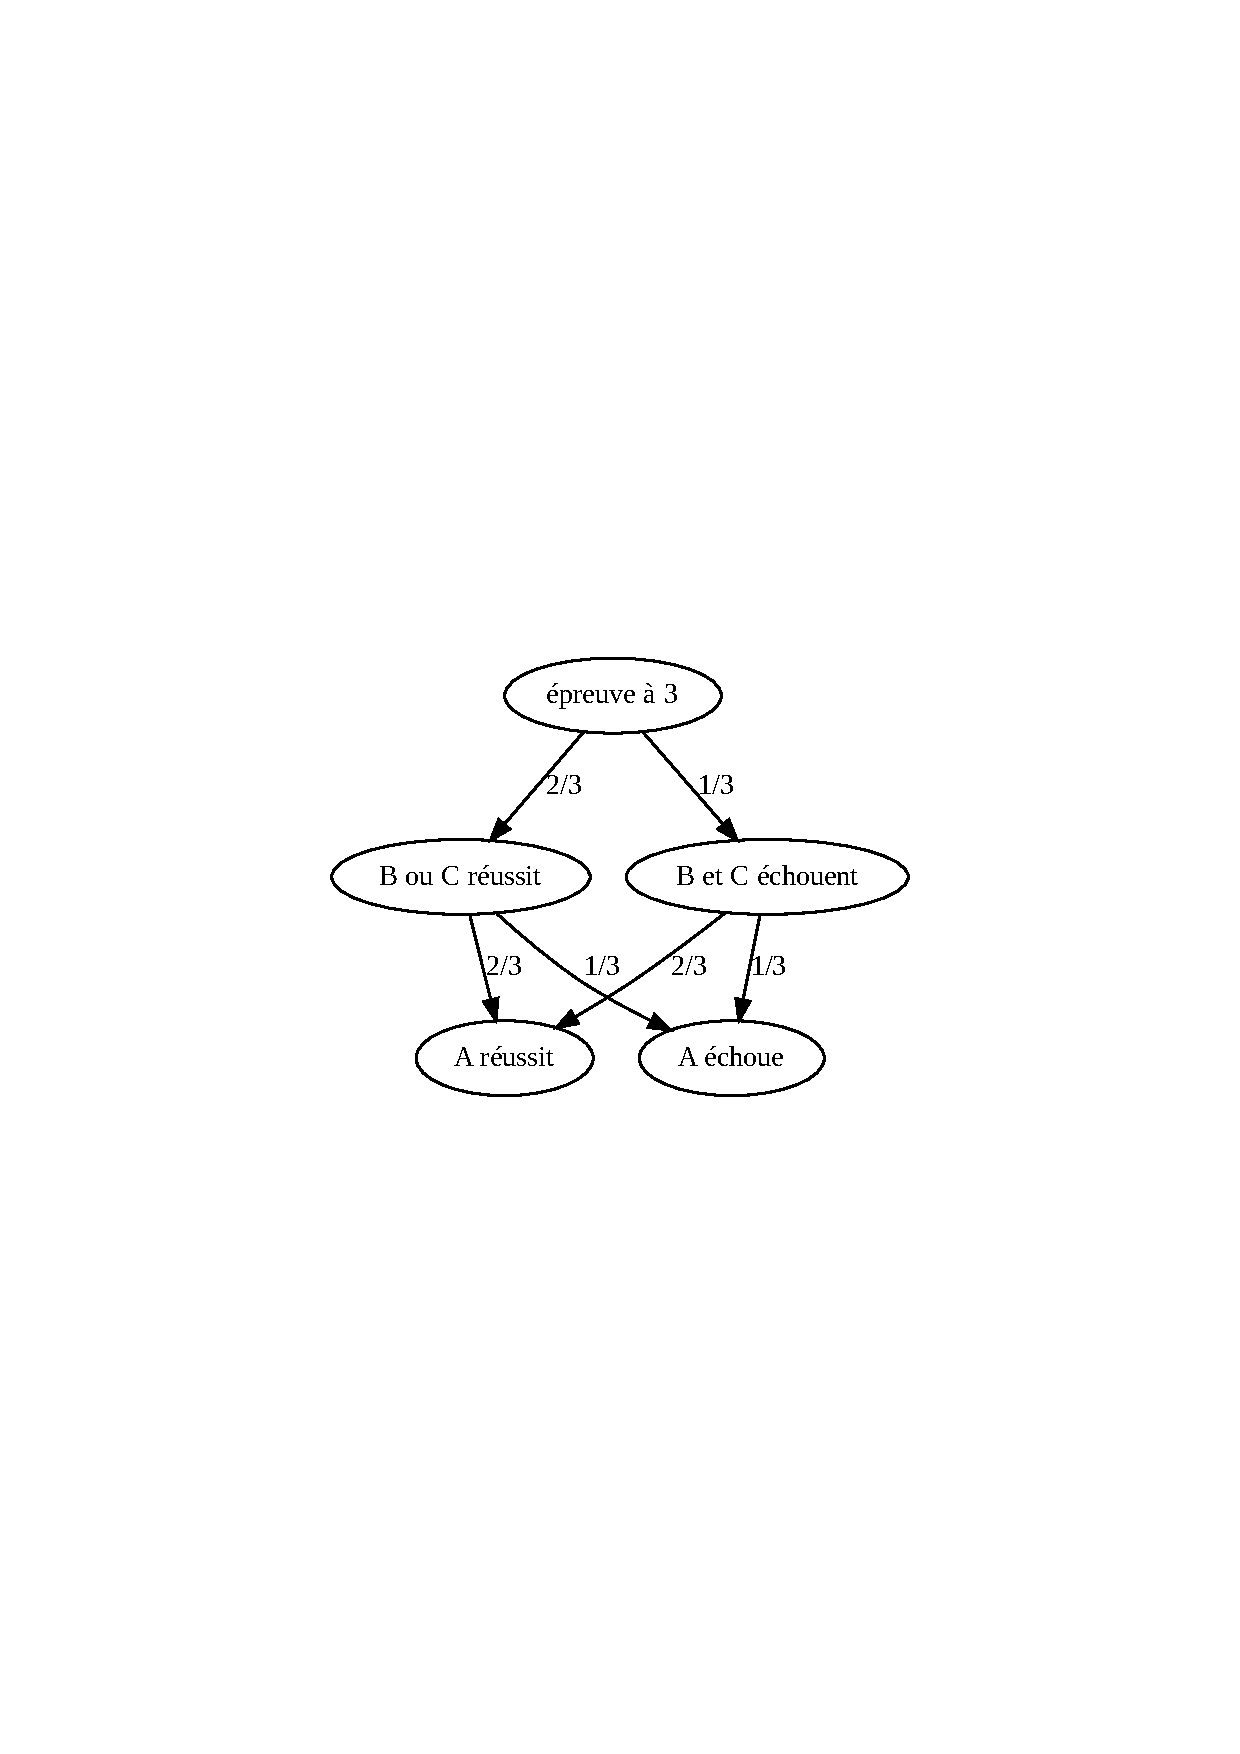
\includegraphics[width=6cm]{Cproba1_1.pdf}
  \caption{probabilités conditionnelles}
  \label{fig:Cproba1_fig1}
\end{figure}

\begin{enumerate}
\item Tant qu'aucun des tireurs n'est éliminé, à chaque étape A vise B,  B et C visent A. Le tireur C n'est pas visé et ne peut donc pas être éliminé avant A ou B. L'événement $AB_n$ est donc impossible.
\item $ABC_{n+1}\cap ABC_n$ est événement $ABC_n$ et \og$A$, $B$ et $C$ ratent leur tir à l'étape $n$\fg. Par indépendance des tirs on a donc 
$$p(ABC_{n+1}|ABC_n)=p (\overline{{\cal A}})p(\overline{{\cal B}})p(\overline{{\cal C}})=\frac 13\frac12\frac23=\frac19$$
\item Comme, tant qu'aucun des tireurs n'est éliminé à chaque étape A vise B,  B et C visent A. L'événement $BC_{n+1}\cap ABC_n$ est événement $ABC_n$ inter l'événement "$A$ rate son tire et  $B$ ou $C$ réussissent   leur tir à l'étape $n$". Par indépendance des tirs on a donc 
$$p(BC_{n+1}|ABC_n)=p (\overline{{\cal A}}\cap({\cal B}\cup {\cal C)})=\frac29 \qquad \text{par 1b)}$$

De même
 $$p(CA_{n+1}|ABC_n)=p ({{\cal A}}\cap\overline{{\cal B}}\cap\overline{ {\cal C}})=\frac 29$$
\item 
\begin{itemize}
\item Si A, B, C ne sont pas éliminés, personne ne vise C, C  ne peut donc pas  être éliminé. D'où
$$p(A_{n+1}|ABC_n)=0 \qquad \text{et}\qquad p(B_{n+1}|ABC_n)=0$$

\item  Comme dans la question précédente 
 $$p(C_{n+1}|ABC_n)= p({\cal A}\cap ({\cal B}\cup {\cal C)})=\frac 49 \qquad \text{par 1c)}$$
\end{itemize}
\item Si à une étape il reste A et C alors A vise sur C et C vise sur A. L'événement $A_{n+1}\cap CA_n$ est donc l'événement $CA_n$ inter l'événement "A rate son tir et C réussit son tir  à l'étape $n$". Par indépendance des tirs, on a donc 
$$p(A_{n+1}|CA_n)= p( {{\cal A}}\cap \overline{{\cal C}})=\frac 49 $$
De même
\begin{displaymath}
p(B_{n+1}|BC_n)= p({{\cal B}}\cap \overline{{\cal C}})=\frac 13\hspace{1cm}
 p(C_{n+1}|CA_{n})= p({{\cal C}}\cap \overline{{\cal A}})=\frac 19  
\end{displaymath}

 et $$p(C_{n+1}|BC_n)= p({{\cal C}}\cap \overline{{\cal B}})=\frac 16$$
\item On a toujours, si A, B, C ne sont pas éliminés, personne ne vise C, C  ne peut donc pas  être éliminé, d'où
$$p(\emptyset_{n+1}|ABC_n)=0$$
D'autre part,
\begin{displaymath}
p(\emptyset_{n+1}|BC_n)= p({{\cal B}}\cap {{\cal C}})=\frac 16
\hspace{1cm} 
p(\emptyset_{n+1}|CA_n)= p({{\cal C}}\cap {{\cal A}})=\frac 29
\end{displaymath}
\end{enumerate} 
\begin{figure}[h!]
  \centering
  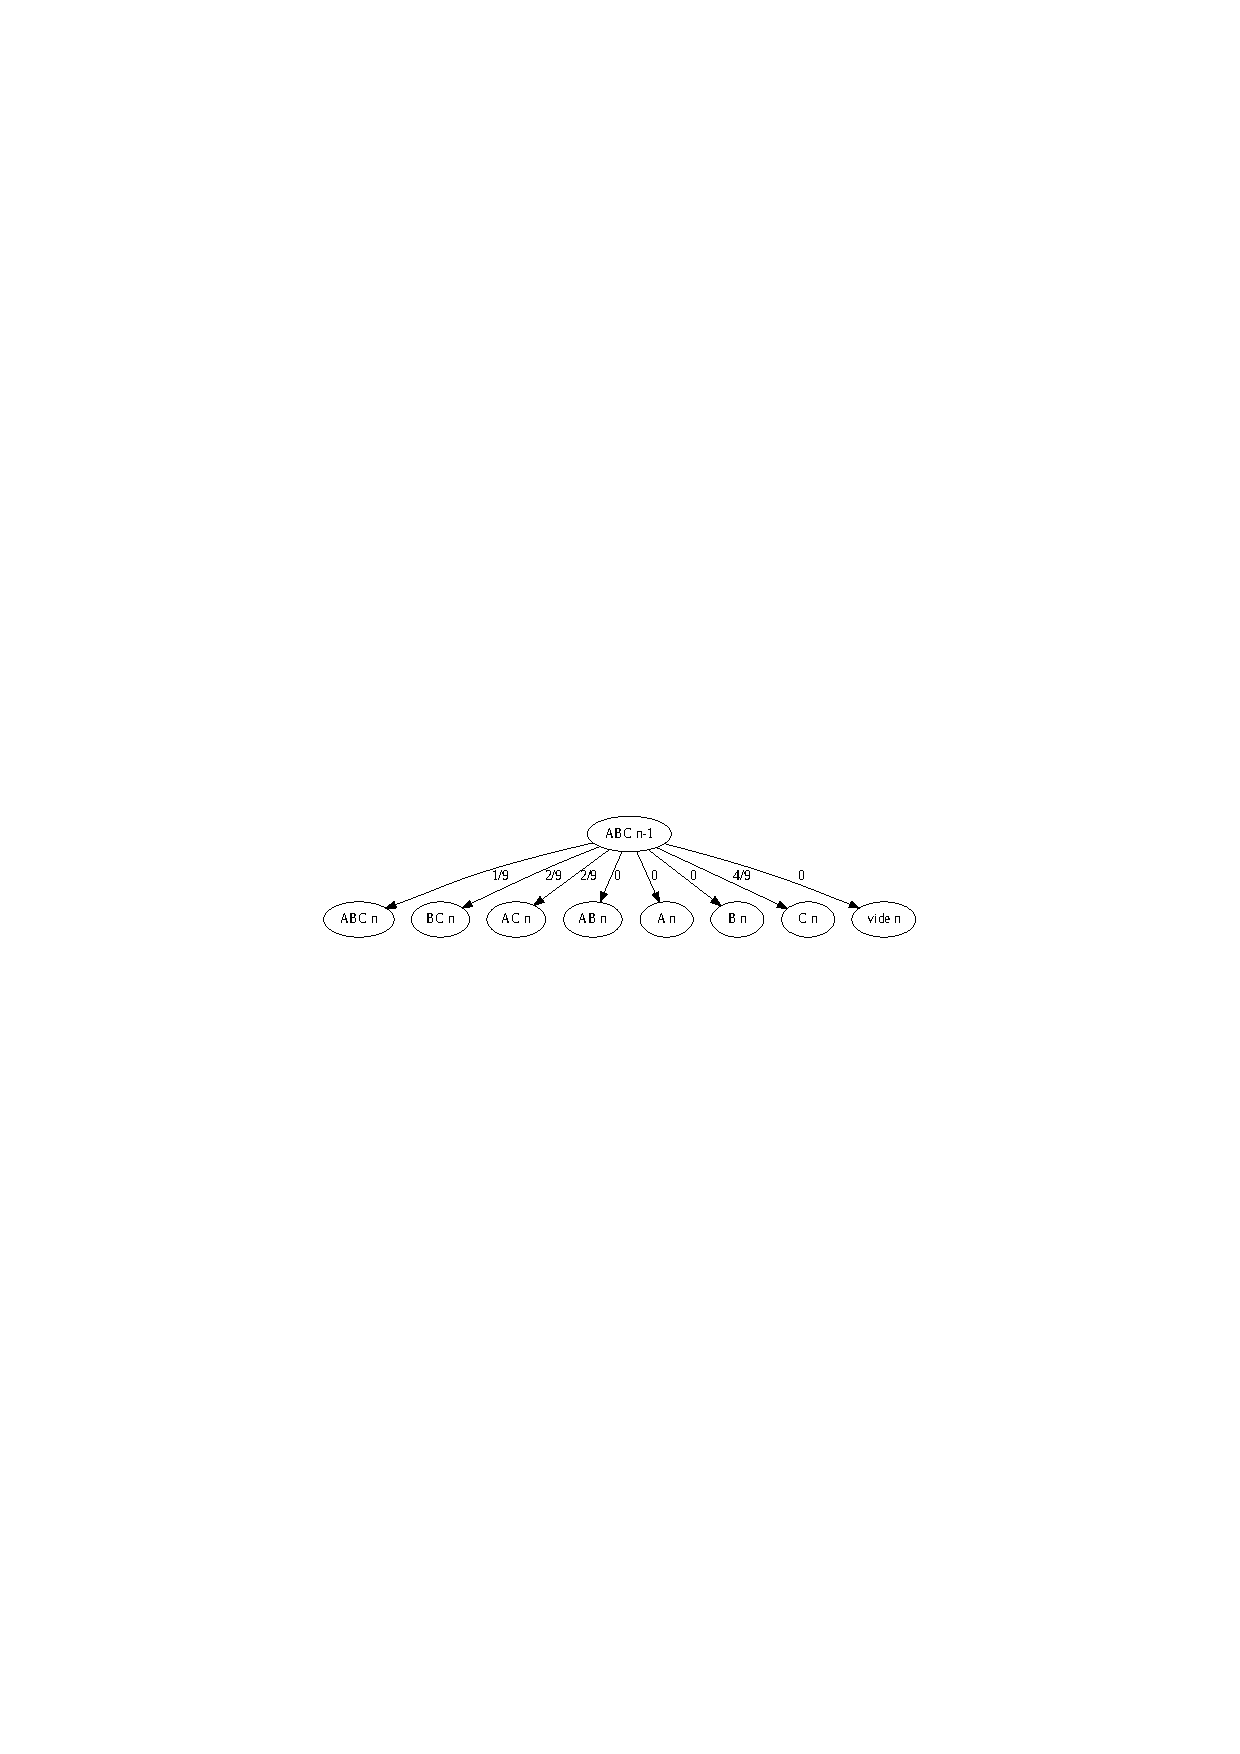
\includegraphics[width=7cm]{./Cproba1_2.pdf}
  \caption{issues épreuve à 3}
  \label{fig:Cproba1_fig2}
\end{figure}

\begin{figure}[h!]
  \begin{minipage}{7cm}
    \centering
    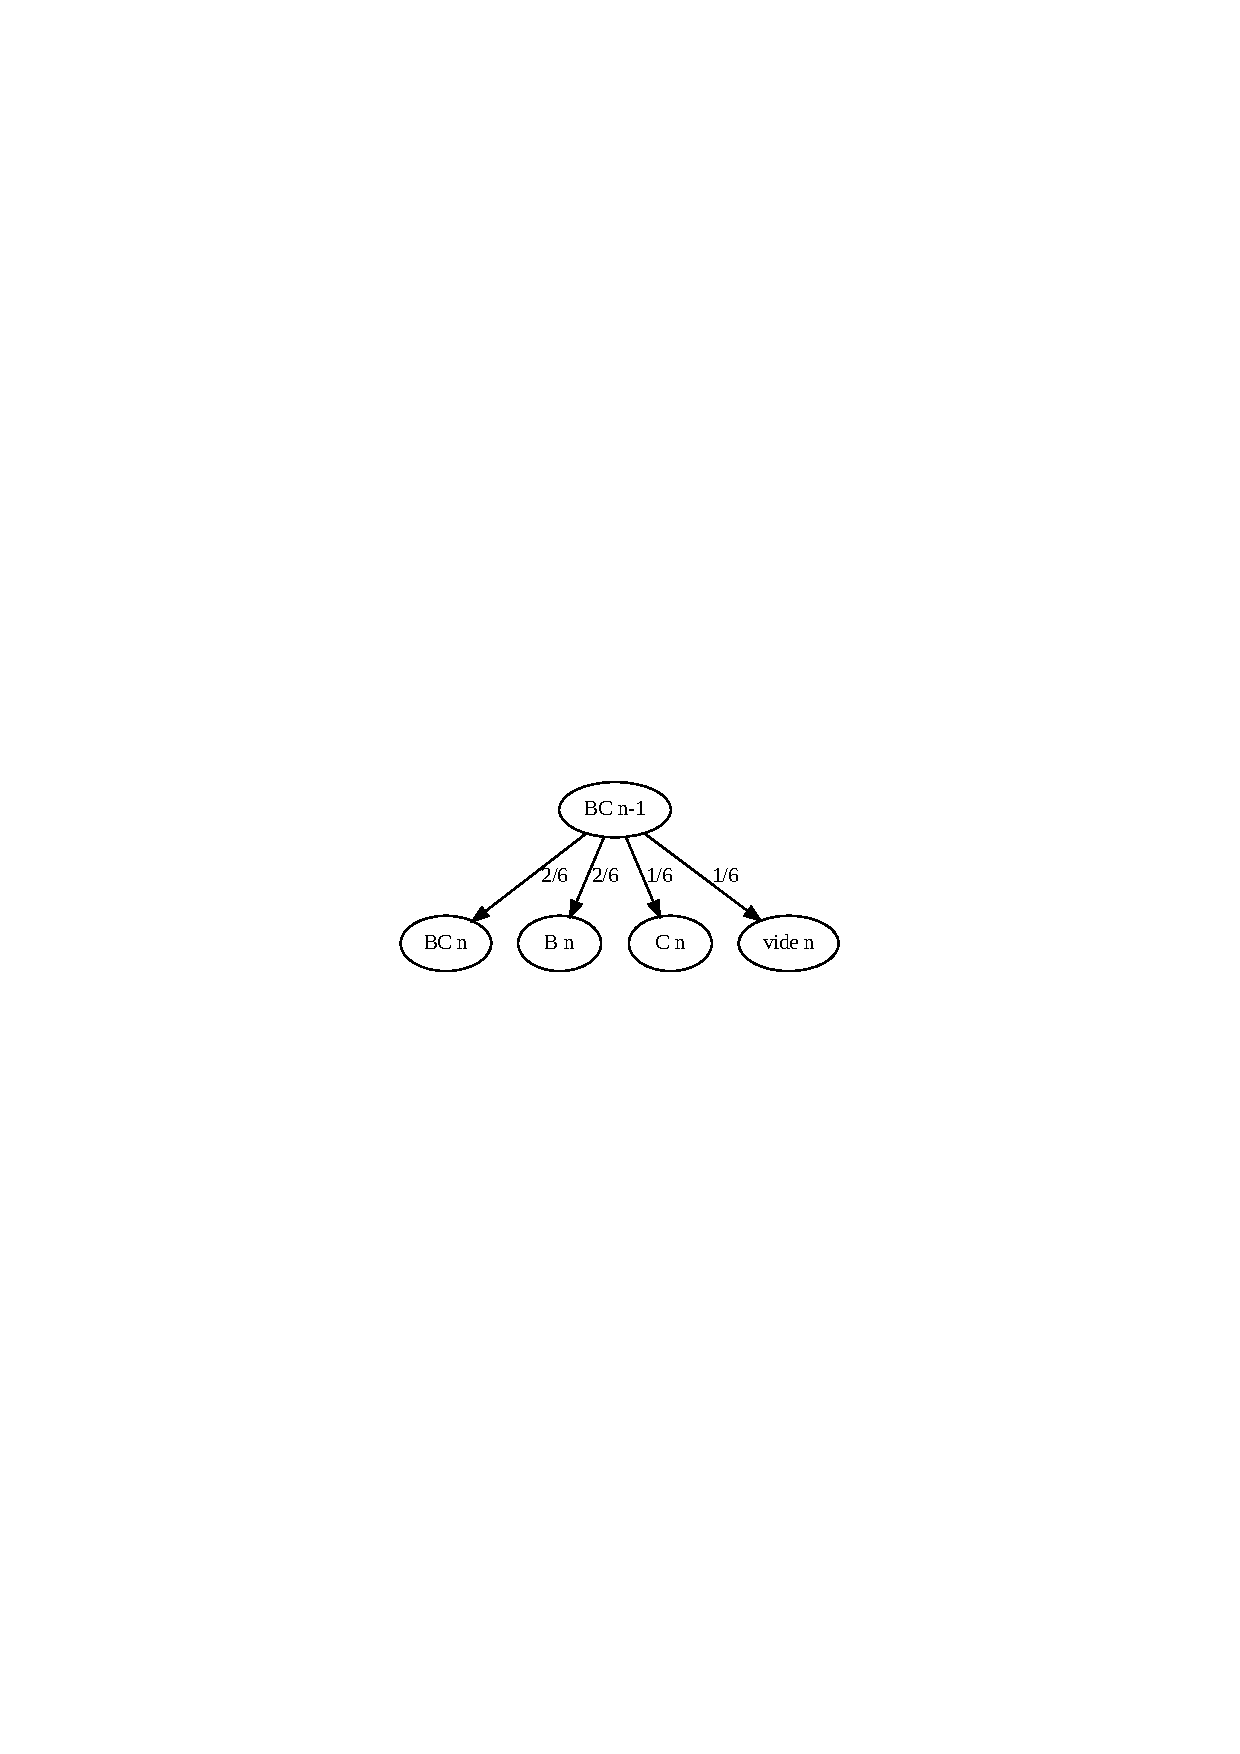
\includegraphics[width=6cm]{./Cproba1_3.pdf}
    \caption{issues épreuve avec BC}
    \label{fig:Cproba1_fig3}
  \end{minipage}
  \begin{minipage}{7cm}
    \centering
    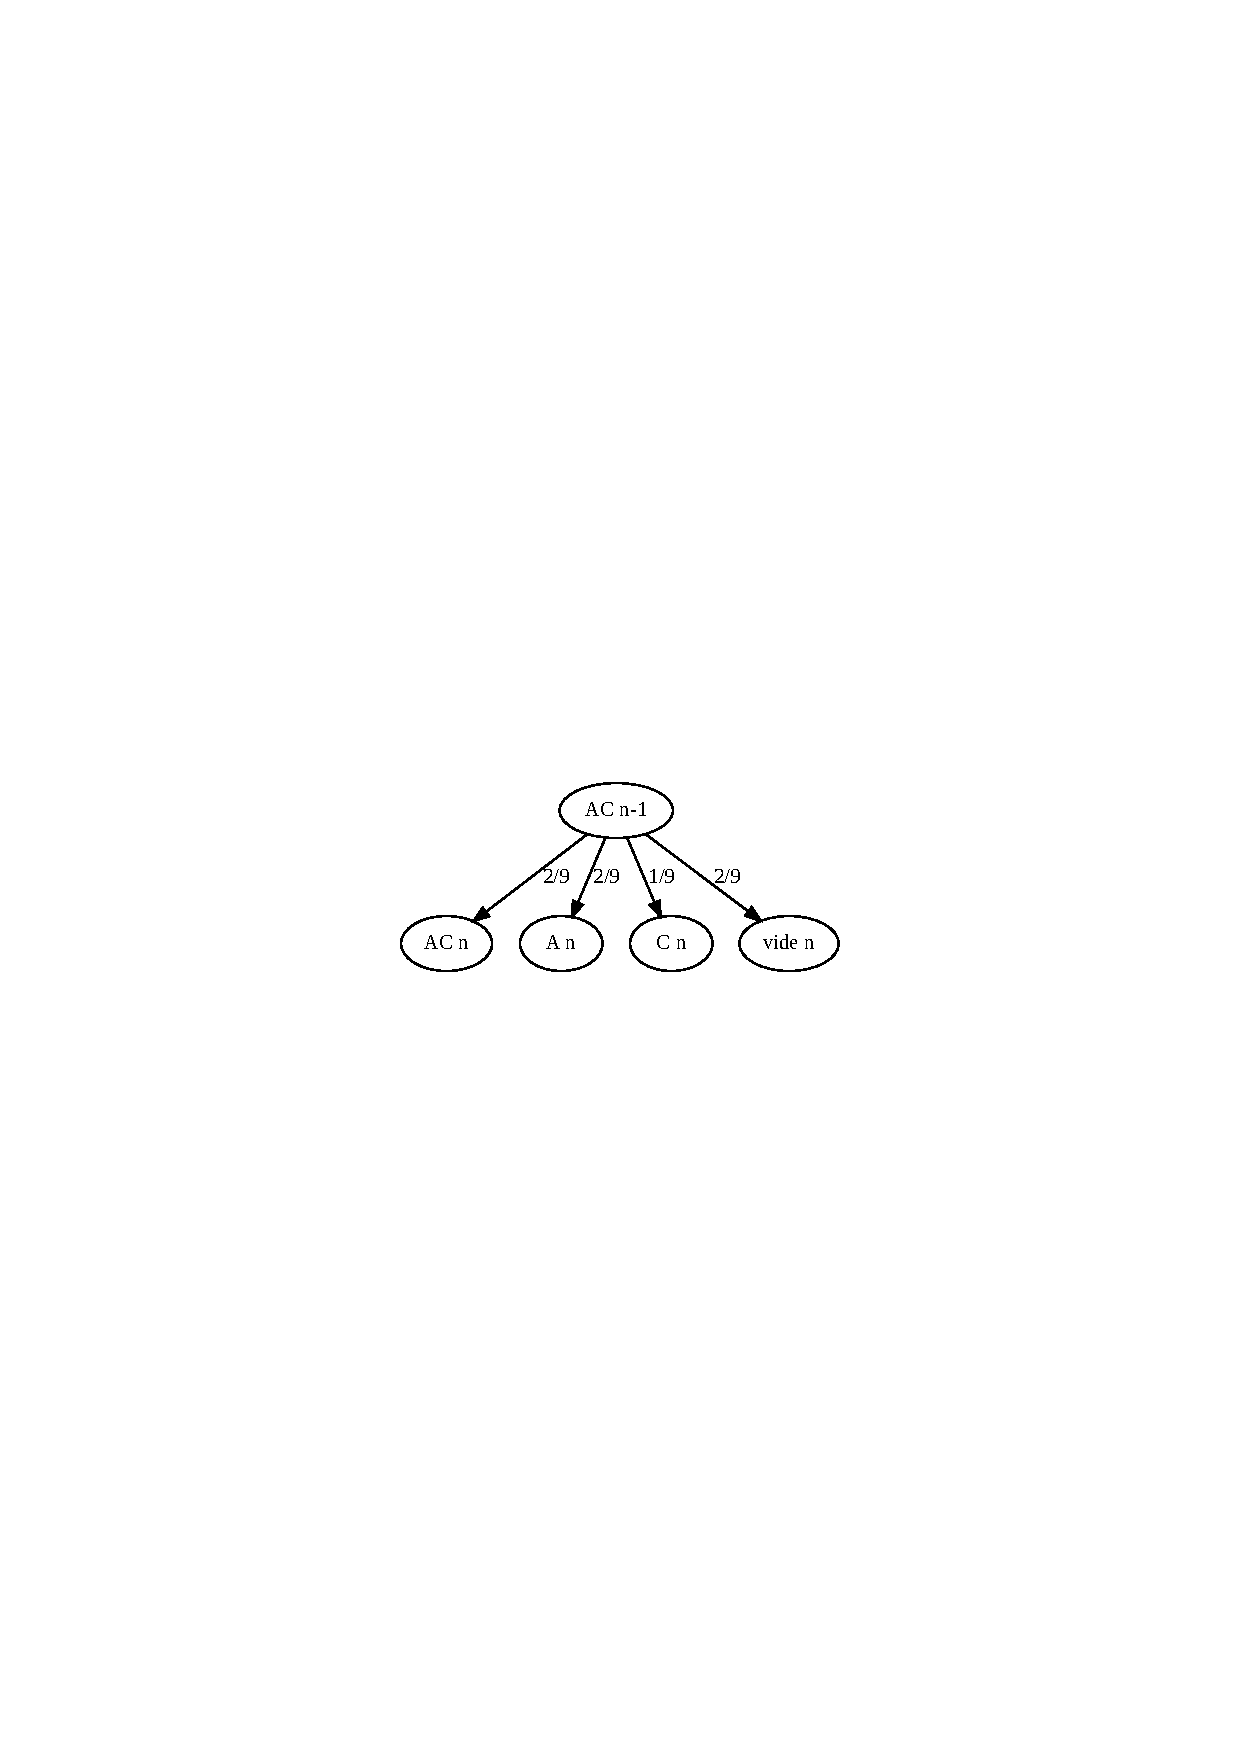
\includegraphics[width=6cm]{./Cproba1_4.pdf}
    \caption{issues épreuve avec AC}
    \label{fig:Cproba1_fig4}
  \end{minipage}
\end{figure}


\item Nombre moyen d'épreuves à l'issue desquelles s'achève le combat.
\begin{enumerate}
\item L'événement $T_1$ est l'union disjointe des événements $A_1$, $B_1$, $C_1$, $\emptyset_{1}$.  La probabilité des événements $A_1$, $B_1$, $C_1$, $\emptyset_{1}$ a été calculé en d) et e) en prenant $n=0$ et en utilisant que $ABC_0$ est l'événement certain. On trouve donc 
$$p(T_1)=p(A_1)+p(B_1)+p(C_1)+p(\emptyset_{1})=0+0+\frac49+0=\frac 49$$
\item Soit $n\se 2$. Remarquons que pour $0\ie k\ie n$
$$ABC_0 \cap ABC_1 \cap \dots \cap ABC_{k-1} \cap ABC_k=ABC_k$$
D'où, par la question 2b.,
\begin{multline*}
p(ABC_1 \cap ABC_2 \cap \dots \cap ABC_{n-1} \cap ABC_n)\\
 = p(ABC_1|ABC_0)p(ABC_2|ABC_1)\dots p(ABC_{n}|ABC_{n-1})= \frac1{9^n}  
\end{multline*}

\item Soit $n \se 2$ et soit $0 \ie k \ie n - 1$, on trouve de même :
\begin{multline*}
p(ABC_1 \cap \dots \cap ABC_k \cap CA_{k+1} \cap \dots \cap CA_n)\\
 = p(ABC_1|ABC_0)\dots p(ABC_{k}|ABC_{k-1})p(CA_{k+1}|ABC_k)\\
  p(CA_{k+2}|CA_{k+1}))\dots p(CA_{n}|CA_{n-1})\\
 = \left(\frac19\right)^k\frac 29 \left(\frac 29\right)^{n-k-1}
 = \frac{2^{n-k}}{9^n}  
\end{multline*}

\item Soit $n \se 2$ et soit $0 \ie k \ie n - 1$ :
\begin{multline*}
p(ABC_1 \cap \dots \cap ABC_k \cap BC_{k+1} \cap \dots \cap BC_n)\\
 = p(ABC_1|ABC_0)\dots p(ABC_{k}|ABC_{k-1})p(BC_{k+1}|ABC_k)\\
  p(BC_{k+2}|BC_{k+1}))\dots p(BC_{n}|BC_{n-1})\\
 = \left(\frac19\right)^k\frac 29 \left(\frac 13\right)^{n-k-1}
 = \frac{2}{3^{n+k+1}}
\end{multline*}

\item Soit $n \se 2$. Notons $T_{>n}$ l'événement étudié. Le combat n'est pas fini à l'issue de la n-ième épreuve si à l'issue de la n-ième épreuve il reste deux ou trois tireurs.  $T_{>n}$ est la réunion disjointe de $ABC_n$, $AB_n$ (qui est l'événement impossible), $CA_n$ et $BC_n$.\\
D'autre part,
\begin{itemize}
\item $CA_n$ est l'union disjointe des événements $ABC_1 \cap \dots \cap ABC_k \cap CA_{k+1} \cap \dots \cap CA_n$, pour $0 \ie k \ie n - 1$ 
\item  $BC_n$ est l'union disjointe des événements $ABC_1 \cap \dots \cap ABC_k \cap BC_{k+1} \cap \dots \cap BC_n$, pour $0 \ie k \ie n - 1$.
 \end{itemize} D'où, d'après les questions b), c) et d)  
\begin{multline*}
p(T_{>n}) = \frac1{9^n}+\sum_{k=0}^{n-1}\frac{2^{n-k}}{9^n}+\sum_{k=0}^{n-1}\frac{2}{3^{n+k+1}}\\
 = \frac1{9^n}+\frac{2^{n+1}-2}{9^n}+\left(\frac1{3^n}-\frac1{9^n}\right)
 = \frac{2^{n+1}+3^n-2}{9^n}
\end{multline*}
On a $T_{>n-1}$ est l'union disjointe de $T_n$ et $T_{>n}$. Donc
$$p(T_n)=p(T_{>n-1})-p(T_{>n})=\frac{2^{n}+3^{n-1}-2}{9^{n-1}}-\frac{2^{n+1}+3^n-2}{9^n}$$
Pour $n=1$, $\frac{2^{n}+3^{n-1}-2}{9^{n-1}}-\frac{2^{n+1}+3^n-2}{9^n}=\frac49$ ce qui correspond à la probabilité de $T_1$.

\item Pour $k\in\N$, posons  $t_k= \frac{2^{k+1}+3^k-2}{9^k}$.\\
 Soit $n\se1$. D'après la formule précédente (valable dès $k=1$)
\begin{multline*}
\sum_{k=1}^n p(T_k)=\sum_{k=1}^n\left(t_{k-1}-t_k\right)
=t_0-t_n \text{ (sommation en dominos) } \\
=1-\frac{2^{n+1}+3^n-2}{9^n}  
\end{multline*}
qui tend bien vers 1 en $+\infty$. D'où
\begin{multline*}
\sum_{k=1}^n kp(T_k)=\sum_{k=1}^n k(t_{k-1}-t_k)=\left(\sum_{k=1}^n t_{k-1}\right)-nt_n \\
  =\left(\sum_{k=0}^{n-1} \frac{2^{k+1}+3^k-2}{9^k}\right)-n\frac{2^{n+1}+3^n-2}{9^n}
\end{multline*}
Ce qui permet de calculer l'espérance:
\begin{displaymath}
\left. 
\begin{aligned}
\sum_{k=0}^{n-1} \frac{2^{k+1}}{9^k} &\text{ tend vers }& \frac{18}{7}\\
\sum_{k=0}^{n-1} \frac{3^{k}}{9^k} &\text{ tend vers }& \frac{3}{2}\\
\sum_{k=0}^{n-1} \frac{2}{9^k} &\text{ tend vers }& \frac{9}{4}\\
n\frac{2^{n+1}+3^n-2}{9^n} &\text{ tend vers }&  0
\end{aligned}
\right\rbrace \Rightarrow 
\sum_{k=1}^n kp(T_k)\text{ tend vers } \frac{51}{28}
\end{displaymath}
\end{enumerate}


\item Probabilités pour que A, B, C remportent le combat
\begin{enumerate}
\item Si A est le seul tireur restant à l'issue de  la n-ième étape alors B et C ont été éliminés avant selon le schéma suivant.
\begin{displaymath}
\text{(ABC)} \xrightarrow{ k \text{ fois }} \text{(ABC)} \rightarrow  \text{(AC)} \xrightarrow{ n-k-2 \text{ fois }}\text{(AC)}\rightarrow \text{(A)}  
\end{displaymath}
Comme déjà vu, tant qu'aucun des tireurs n'est éliminé à chaque étape A vise B,  B et C visent A. B est donc éliminé (strictement) avant C. Dès que C est éliminé, A gagne. On voit donc que l'événement $A_1$ est impossible et que  pour $n\se 2$, $A_n$ est l'union disjointe des $$ABC_1 \cap \dots \cap ABC_k \cap CA_{k+1} \cap \dots \cap CA_{n-1} \cap A_n$$ pour $0 \ie k \ie n - 2$ (où $k$ correspond à l'étape où B a été éliminé). 
\item Soit $n\se 2$ et  $0 \ie k \ie n - 2$. D'après la formule des probabilités composées, la probabilité de l'événement correspondant au schéma indiqué est
\begin{displaymath}
  \left( \frac{1}{9}\right)^{k}\times \frac{2}{9} \times \left( \frac{2}{9}\right)^{n-k-2}\times \frac{4}{9} = \frac{1}{9^n}2^{n+1-k}
\end{displaymath}
Ces événements indexés par $k$ sont disjoints, la probabilité que A remporte le combat à l'issue de l'épreuve $n$ est donc la somme des probabilités
\begin{displaymath}
  \sum_{k=0}^{n-2}\frac{1}{9^n}2^{n+1-k} = \frac{1}{9^n}\left(2^{n+1}+\cdots+2^3 \right) = \frac{2^{n+2} -2^{3}}{9^{n}}
  =4\left(\frac{2}{9} \right)^{n}-8\left(\frac{1}{9} \right)^{n} 
\end{displaymath}

\item L'événement A est l'union disjointe des $A_n$ pour $n\se2$. Donc $p(A)$ est la limite quand $n$ tend vers $+\infty$ de  
$\sum_{k=2}^n p(A_k)$. On obtient $p(A)=\frac{1}{63}PB$.
\begin{displaymath}
  p(A) = 4\left(\frac{2}{9} \right)^{2}\frac{1}{1-\frac{2}{9}}- 8\left(\frac{1}{9} \right)^{2}\frac{1}{1-\frac{1}{9}}
  =\frac{16}{9\times 7} - \frac{8}{9\times 8}=\frac{16-7}{9\times 7}=\frac{1}{7}
\end{displaymath}


\item Suivant  le même principe $B_n$ est l'union disjointe, pour $0 \ie k \ie n - 2$, des 
$$ABC_1 \cap \dots \cap ABC_k \cap BC_{k+1} \cap \dots \cap BC_{n-1} \cap B_n$$
Soit $n\se 2$ et  $0 \ie k \ie n - 2$
\begin{multline*}
p(ABC_1 \cap \dots \cap ABC_k \cap BC_{k+1} \cap \dots \cap BC_{n-1} \cap B_n)\\
 = p(ABC_1 \cap \dots \cap ABC_k \cap BC_{k+1} \cap \dots \cap BC_{n-1})p(B_n|BC_{n-1})\\
 = \frac 2{3^{n+k}}\frac 13=\frac{2}{3^{n+k+1}}
\end{multline*}
D'où
$$p(B_n)=\frac1{3^n}-\frac1{3^{2n-1}}$$
Donc $p(B)$ est la limite quand $n$ tend vers $+\infty$ de  
$\sum_{k=2}^n p(B_k)$. On obtient 
\begin{displaymath}
  p(B) = \left(\frac{1}{3} \right)^{2}\frac{1}{1-\frac{1}{3}}- 3\left(\frac{1}{9} \right)^{2}\frac{1}{1-\frac{1}{9}}
  =\frac{1}{8}
\end{displaymath}
\item Pour que C gagne le combat à l'étape $n$ il y a plusieurs cas de figure :
\begin{itemize}
\item Soit A et B sont éliminés en même temps. Notons $C_{n,AB}$ cet événement.\\
C'est aussi $ABC_1\cap\dots\cap ABC_{n-1}\cap C_n$ de probabilité $$p(ABC_1\cap\dots\cap ABC_{n-1}\cap C_n)=p(ABC_{n-1})p(C_n|ABC_{n-1})=\frac{1}{9^{n-1}}\frac 49=\frac4{9^{n}}$$

\item Soit A est  éliminé puis B. Notons $C_{n,B}$ cet événement.\\
C'est l'union disjointe, pour  $0 \ie k \ie n - 2$, des événements  
$$ABC_1 \cap \dots \cap ABC_k \cap BC_{k+1} \cap \dots \cap BC_{n-1} \cap C_n$$
Soit $n\se 2$ et  $0 \ie k \ie n - 2$
\begin{multline*}
p(ABC_1 \cap \dots \cap ABC_k \cap BC_{k+1} \cap \dots \cap BC_{n-1} \cap C_n)\\
 = p(ABC_1 \cap \dots \cap ABC_k \cap BC_{k+1} \cap \dots \cap BC_{n-1})p(C_n|BC_{n-1}))\\
 = \frac 2{3^{n+k}}\frac 16=\frac{1}{3^{n+k+1}}  
\end{multline*}
La probabilité de $C_{n,B}$ est donc :
$$\frac12(\frac1{3^n}-\frac1{3^{2n-1}})$$

\item Soit B est éliminé puis A. Notons $C_{n,A}$ cet événement. C'est l'union disjointe, pour $0 \ie k \ie n - 2$, des événements  
$$ABC_1 \cap \dots \cap ABC_k \cap CA_{k+1} \cap \dots \cap CA_{n-1} \cap C_n$$
Soit $n\se 2$ et  $0 \ie k \ie n - 2$
\begin{multline*}
p(ABC_1 \cap \dots \cap ABC_k \cap CA_{k+1} \cap \dots \cap CA_{n-1} \cap C_n)\\
 = p(ABC_1 \cap \dots \cap ABC_k \cap CA_{k+1} \cap \dots \cap CA_{n-1})p(C_n|CA_{n-1})\\
 = \frac{2^{n-k-1}}{9^{n-1}}\frac 19=\frac{2^{n-1-k}}{9^n}
\end{multline*}
 
La probabilité de  $C_{n,A}$ est donc 
$$\sum_{k=0}^{n-2}\frac{2^{n-1-k}}{9^n}=\frac{1}{9^n}(2^{n}-2)$$
\end{itemize}

L'événement $C_n$ est l'union disjointe des $C_{n,AB}$, $C_{n,B}$ et $C_{n,A}$ 
Donc $p(C)$ est la limite quand $n$ tend vers $+\infty$ de  
\begin{displaymath}
\sum_{k=1}^n p(C_{n,AB})+\sum_{k=2}^np(C_{n,B})+\sum_{k=2}^np(C_{n,A})  
\end{displaymath}
On obtient:
\begin{displaymath}
\left. 
\begin{aligned}
&\sum_{k=1}^n p(C_{n,AB}) &\text{ tend vers }& \frac 12\\
&\sum_{k=2}^n p(C_{n,B}) &\text{ tend vers }& \frac 1{16}\\
&\sum_{k=2}^n p(C_{n,A}) &\text{ tend vers }& \frac 1{28}
\end{aligned}
\right\rbrace 
\Rightarrow p(C)=\frac {67}{112}
\end{displaymath}

\end{enumerate}
\end{enumerate} 


\subsection*{PARTIE II}
\begin{enumerate}

\item  Expression de la matrice de transition $M$
\begin{enumerate}
\item  On trouve
\begin{displaymath}
\renewcommand{\arraystretch}{2}
M=
\begin{pmatrix}
\dfrac19&0&0&0&0&0&0\\
\dfrac 29&\dfrac 13&0&0&0&0&0\\
\dfrac29&0&\dfrac29&0&0&0&0\\
0&0&\dfrac49&1&0&0&0\\
0&\dfrac 13& 0&0&1&0&0\\
\dfrac 49&\dfrac 16&\dfrac 19&0&0&1&0\\
0&\dfrac16&\dfrac29&0&0&0&1
\end{pmatrix}  
\end{displaymath}

\item Soit $n\in\N$. Par récurrence, $E_n=M^nE_0$. 
\end{enumerate}

\item  Calcul des puissances de la matrice $M$.

\begin{enumerate}
\item Vérification évidente à l'aide du produit par blocs.
\item En lisant dans la matrice de transition, on trouve
\begin{displaymath}
\renewcommand{\arraystretch}{2}
U= 
\begin{pmatrix}
\dfrac19  & 0        & 0\\
\dfrac 29 & \dfrac 13 & 0\\
\dfrac29  & 0        &\dfrac29\\    
\end{pmatrix}
\hspace{1cm}
V=
\begin{pmatrix}
0&0&\dfrac49\\
0&\dfrac 13& 0\\
\dfrac 49&\dfrac 16&\dfrac 19\\
0&\dfrac16&\dfrac29
\end{pmatrix}
\end{displaymath}

\item  
\end{enumerate}
\item  Diagonalisation de la matrice $U$
\begin{enumerate}
\item Le système considéré admet une solution non nulle si la matrice $U-\lambda I_3$ n'est pas inversible. Notons $P(\lambda)$ le déterminant de cette matrice.
\begin{displaymath}
\renewcommand{\arraystretch}{1.6}
P(\lambda)=
\begin{vmatrix}
\frac19-\lambda&0&0\\
\frac 29&\frac 13-\lambda&0\\
\frac29&0&\frac29-\lambda\\
\end{vmatrix}=(\frac19-\lambda)(\frac 13-\lambda)(\frac29-\lambda)  
\end{displaymath}
D'où $\lambda_1=\frac 19$, $\lambda_2=\frac 29$ et $\lambda_3=\frac 13$.\\
La résolution des systèmes donne $V_1=(1,-1,-2)$, $V_2=(0,0,1)$ et $V_3=(0,1,0)$.
\item  D'après la formule de changement de base, on obtient le résultat cherché, en formant la matrice des vecteurs propres trouvés soit: 
\begin{displaymath} \renewcommand{\arraystretch}{2}
P = 
\begin{pmatrix}
1&0&0\\
-1&0& 1\\
-2&1&0      
\end{pmatrix}
\hspace{0.5cm}\text{ et }\hspace{0.5cm}
D = 
\begin{pmatrix}
\frac{1}{9} & 0 & 0 \\
0&\frac 29& 0\\
0&0&\frac 13  
\end{pmatrix}
\hspace{0.5cm}\text{ avec }\hspace{0.5cm}
P^{-1}=\begin{pmatrix}
1&0&0\\2&0& 1\\
1&1&0
\end{pmatrix}  
\end{displaymath}
\end{enumerate}

\item  Calcul de la limite des puissances de la matrice $M$.
\begin{enumerate}
\item Soit $n\in\N$, $$D^n=\left(\begin{array}{ccc}
\frac 1{9^n}&0&0\\
0&\frac {2^n}{9^n}& 0\\
0&0&\frac 1{3^n}
\end{array}\right)$$ et $$I_3+D+\dots+D^n=\left(\begin{array}{ccc}
\frac 98-\frac 1{8.9^n}&0&0\\
0&\frac 97-\frac{2^{n+1}}{7.9^n}& 0\\
0&0&\frac 32-\frac 1{2.3^n}
\end{array}\right)$$

\item On obtient que $(D^n)$ converge vers la matrice nulle et que $(I_3+D+\dots+D^n)$ converge vers la matrice
\begin{displaymath}
\renewcommand{\arraystretch}{1.5}
\begin{pmatrix}
\dfrac 98&0&0\\
0&\dfrac 97& 0\\
0&0&\dfrac 32
\end{pmatrix}  
\end{displaymath}

De $U=PDP^{-1}$, on tire $U^n=PD^nP^{-1}$ pour $n\in\N$. On en déduit que $(U^n)$ converge vers $P0P^{-1}$ ie vers la matrice nulle
et $(I_3+U+\dots+U^n)$ converge vers la matrice 
\begin{displaymath}
\renewcommand{\arraystretch}{1.9}
P \begin{pmatrix}
\dfrac 98&0&0\\
0&\dfrac 97& 0\\
0&0&\dfrac 32
\end{pmatrix}P^{-1}
=\begin{pmatrix}
\dfrac 98&0&0\\
\dfrac 38&\dfrac 32& 0\\
\dfrac 9{28}&0&\dfrac 97
\end{pmatrix}
\end{displaymath}

\item D'après l'expression de $M^n$ trouvée en 2)c) et en utilisant que $(V+VU+\dots+VU^n)$ converge vers la matrice
\renewcommand{\arraystretch}{1.9}
 $$V\left(\begin{array}{ccc}
\dfrac 98&0&0\\
\dfrac 38&\frac 32& 0\\
\dfrac 9{28}&0&\dfrac 97
\end{array}\right)=\left(\begin{array}{ccc}
\dfrac 1{7}&0&\dfrac 47\\
\dfrac 18&\frac 12& 0\\
\dfrac {67}{112}&\dfrac 14&\dfrac 17\\
\dfrac {15}{112} &\dfrac 14&\dfrac 27
\end{array}\right)$$

Donc $$E_n=M^nE_0=\left(\begin{array}{c}
0\\
0\\
0\\
\dfrac 1{7}\\
\dfrac 18\\
\dfrac {67}{112}\\
\dfrac {15}{112}
\end{array}\right)$$
\item On retrouve bien que $(p(ABC_n))$, $(p(BC_n))$ et $(p(CA_n))$ convergent vers $0$, que $(p(A_n))$ converge vers $\dfrac 1{7}$, que $(p(B_n))$ converge vers $\dfrac 18$, que $(p(C_n)$ converge vers $\dfrac {67}{112}$ et que $(p(\emptyset_n)$ converge vers $\dfrac {15}{112}$.
\end{enumerate}
\end{enumerate} 



